\documentclass[a4paper,onecolumn]{article}
\usepackage[page,toc,titletoc,title]{appendix}
\usepackage{url}
\usepackage{subfigure}
\usepackage[sc]{mathpazo} % Use the Palatino font
\usepackage[T1]{fontenc} % Use 8-bit encoding that has 256 glyphs
\usepackage[utf8]{inputenc} % Use utf-8 as encoding
\linespread{1.05} % Line spacing - Palatino needs more space between lines
\usepackage{microtype} % Slightly tweak font spacing for aesthetics
\usepackage[spanish, activeacute]{babel}
 \decimalpoint
% \usepackage[hmarginratio=1:1,top=32mm,columnsep=20pt]{geometry} % Document marginshttps://www.overleaf.com/project/60211b96f72a79d4c7515e93
% \usepackage[hang, small,labelfont=bf,up,textfont=it,up]{caption} % Custom captions under/above floats in tables or figures
\usepackage{verbatim} % comentarios
\usepackage{listings}
\lstset{
frame=single,
breaklines=true,
numbers=left,
keywordstyle=\color{blue},
numbersep=5pt,
numberstyle=,
basicstyle=\linespread{1.5}\selectfont\ttfamily,
commentstyle=\color{gray},
stringstyle=\color{orange},
identifierstyle=\color{green!40!black},
}
\lstdefinestyle{console}
{
numbers=left,
backgroundcolor=\color{violet},
%belowcaptionskip=1\baselineskip,
breaklines=true,
%xleftmargin=\parindent,
%showstringspaces=false,
basicstyle=\footnotesize\ttfamily,
%keywordstyle=\bfseries\color{green!40!black},
%commentstyle=\itshape\color{green},
%identifierstyle=\color{blue},
%stringstyle=\color{orange},
basicstyle=\scriptsize\color{white}\ttfamily,
}
\setlength{\parskip}{0.8em}
\usepackage{natbib}
\usepackage{enumitem}
% \setlist[itemize]{noitemsep} % Make itemize lists more compact
% \usepackage{abstract} % Allows abstract customization
% \renewcommand{\abstractnamefont}{\normalfont\bfseries} % Set the "Abstract" text to bold
% \renewcommand{\abstracttextfont}{\normalfont\small\itshape} % Set the abstract itself to small italic text
\usepackage{titlesec}

\usepackage{fancyhdr} % Headers and footers
\pagestyle{fancy} % All pages have headers and footers
\fancyhead{}
\lhead{Hugo Gómez Sabucedo}
\rhead{Bases de datos SQL}

\renewcommand{\footrulewidth}{0.2pt}
\usepackage{titling} % Customizing the title section
\usepackage[breaklinks=true]{hyperref} % For hyperlinks in the PDF
%\usepackage{array}
%\newcolumntype{C}[1]{>{\centering\let\newline\\\arraybackslash\hspace{0pt}}m{#1}}
\usepackage{graphicx}
%\usepackage{lipsum} % NO NECESARIO LUEGO
%\usepackage{xcolor} % NO NECESARIO LUEGO
%\usepackage{amsmath}
%\usepackage{wrapfig}
%\usepackage{multicol}
%\usepackage{bm}


\let\stdsection\section
\renewcommand\section{\newpage\stdsection}

%-------------------------------------------------------------------------------
%	TITLE SECTION
%-------------------------------------------------------------------------------

\setlength{\droptitle}{-4\baselineskip} % Move the title up



\title{\begin{center} \Huge Bases de datos SQL \end{center}} % Article title
\author{
    \textsc{\Huge Hugo Gómez Sabucedo} \\ % Your name
    \large \href{mailto:hugogomezsabucedo@gmail.com}{hugogomezsabucedo@gmail.com} \\ [2ex] % Your email address
    \Large \textbf{Máster Big Data, Data Science \& Inteligencia Artificial} \\
    \normalsize Curso 2024-2025 \\
    \large Universidad Complutense de Madrid
}
\date{} % Leave empty to omit a date

\begin{document}
% Print the title
\maketitle
%tableofcontents
\begin{sloppypar}

%-------------------------------------------------------------------------
%	DOCUMENT
%-------------------------------------------------------------------------

\section{Enunciado del problema} \label{enunciado}
El enunciado del problema es el siguiente:

Tenemos una empresa dedicaba a la organización de eventos culturales únicos “ArteVida Cultural”. Organizamos desde deslumbrantes
conciertos de música clásica hasta exposiciones de arte vanguardista, pasando por apasionantes obras de teatro y cautivadoras
conferencias, llevamos la cultura a todos los rincones de la comunidad.

Necesitamos gestionar la gran variedad de eventos y detalles, así como las ganancias que obtenemos. Para ello, es
necesario llevar un registro adecuado de cada evento, de los artistas que los protagonizan, las ubicaciones donde
tienen lugar, la venta de entradas y, por supuesto, el entusiasmo de los visitantes que asisten.

Hemos decidido diseñar e implementar una base de datos relacional que no solo simplifique la organización de
eventos, sino que también permita analizar datos valiosos para tomar decisiones informadas.

En nuestra empresa ofrecemos una serie de actividades que tienen un nombre, un tipo: concierto de distintos tipos
de música (clásica, pop, blues, soul, rock and roll, jazz, reggaeton, góspel, country, …), exposiciones, obras de teatro
y conferencias, aunque en un futuro estamos dispuestos a organizar otras actividades. Además, en cada actividad
participa uno o varios artistas y un coste (suma del caché de los artistas).

El artista tiene un nombre, un caché que depende de la actividad en la que participe y una breve biografía.

La ubicación tendrá un nombre (Teatro Maria Guerrero, Estadio Santiago Bernabeu, …), dirección, ciudad o pueblo,
aforo, precio del alquiler y características.

De cada evento tenemos que saber el nombre del evento (p.e. “VI festival de música clásica de Alcobendas”), la
actividad, la ubicación, el precio de la entrada, la fecha y la hora, así como una breve descripción del mismo. En un
evento sólo se realiza una actividad.

También tendremos en cuenta los asistentes a los eventos, de los que sabemos su nombre completo, sus teléfonos
de contacto y su email. Una persona puede asistir a más de un evento y a un evento pueden asistir varias personas.

Nos interesará realizar consultas por el tipo de actividad, en que fecha se han realizado más eventos, en qué ciudad
realizamos más eventos, …

\section{Diseño conceptual} \label{mer}
El diagrama entidad-relación que se propone es el siguiente:
\begin{center}
    \begin{figure}[h!]
        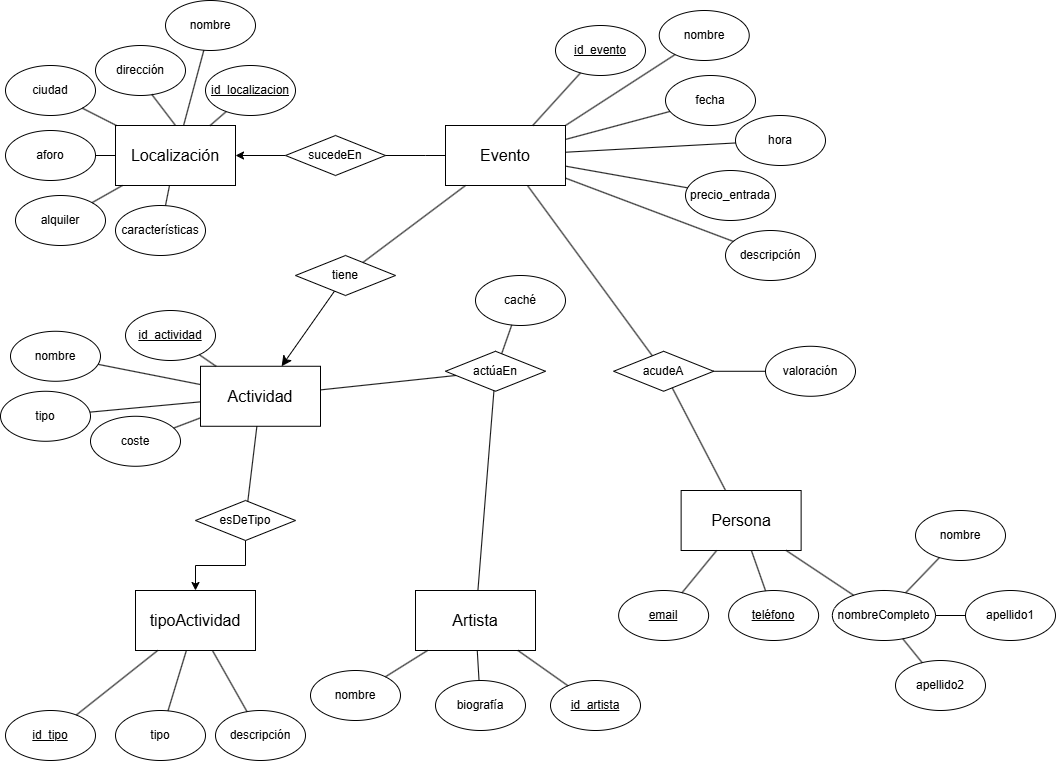
\includegraphics[width=\textwidth]{MER.png}
    \end{figure}
\end{center}

A continuación se explica más en profundidad dicho diagrama y las diferentes entidades y relaciones que lo componen.

En resumen, se han definido seis entidades (actividad, tipoActividad, artista, evento, localización y persona), cada una de las 
cuales se corresponde con los principales conceptos que se mencionan en el enunciado del ejercicio. Además, se han definido
cinco relaciones (sucedeEn, tiene, actúaEn, acudeA y esDeTipo) entre las entidades anteriormente mencionadas.

En primer lugar tenemos la entidad \textbf{Evento}, que representa cada uno de los eventos que realiza la empresa. Esta entidad tendrá como atributos
el nombre, la fecha y hora (que en este punto he considerado como dos atributos diferenciados, aunque a posteriori en el paso a tablas pueda
definirse como un único atributo, por ejemplo, de tipo \textit{timestamp}), el precio de la entrada y la descripción del mismo. Además, se ha
añadido un atributo adicional, \underline{id\_evento}, el cual se usará como clave primaria de la entidad. Aunque incialmente había pensado en 
utilizar como clave del evento su nombre y la fecha y hora, no me parece la mejor decisión, también en terminos de rendimiento.

Un evento tiene lugar en una ubicación en concreto. Es por eso que se define la entidad \textbf{Localización}, que representa las diferentes
salas o lugares donde puede tener lugar un evento. Como se indica, sus atributos son su nombre, la dirección, la ciudad, el aforo,
el precio del alquiler y las características del mismo. A mayores, se ha definido un atributo adicional \underline{id\_localizacion},
el cual, al igual que en el caso anterior, usaremos como clave primaria de la entidad.

Entre estas dos entidades surge la relación \textbf{sucedeEn}, que es de 1 a muchos entre Evento y Localización, ya que un evento sólamente puede
tener lugar en una localización, pero una misma localización puede albergar varios eventos a lo largo del tiempo.

Por una parte, se define la entidad \textbf{Persona}, que representa los diferentes asistentes a los eventos. De éstas, únicamente se nos indica 
que nos interesan su nombre completo, su email y su teléfono. El nombre completo lo hemos definido como un atributo compuesto, el cual dividimos
a su vez en nombre, apellido1 y apellido2. Por su parte, como clave primaria se ha considerado el \underline{email} y el \underline{teléfono} de la 
persona. En el enunciado del problema no se especifica que se vayan a recoger identificadores únicos de las personas, como podría ser el DNI, por lo que
este no se puede añadir como atributo. Además, emplear un identificador autogenerado y autoincremental me parecía redundante respecto al resto de 
entidades, y poco eficiente. Por eso he considerado el email y teléfono como la clave primaria, ya que me parece que es una combinación que, en cualquier
caso, debería ser única (no tendría mucho sentido que una persona se registrase varias veces pero con diferentes combinaciones de email y teléfono).

Esta entidad tiene únicamente una relación, \textbf{acudeA}, que la relaciona con el evento. Esta relación es de muchos a muchos, ya que se indica que una persona
puede asistir a varios eventos, y que a un evento asisten varias personas. Además, en el enunciado se comenta que para los eventos se desea conocer
"el entusiasmo de los visitantes que asisten". Es por ello que se ha definido un atributo de esta relación, valoración, que nos permitirá registrar
las opiniones de los asistentes a los diferentes eventos.

Por otra parte, se define la entidad \textbf{Actividad}, que se corresponde con cada una de las diferentes actividades que tienen lugar en el evento.
Como se indica, de una actividad nos interesa su nombre, su tipo y su coste. Adicionalmente, se define el atributo \underline{id\_actividad}, para 
establecerlo como clave primaria de la entidad. Respecto al coste de la actividad, se indica que el coste es la suma del caché de los artistas. 
Este coste, en el modelo entidad relación, se ha definido como un atributo diferenciado, pero es importante destacar que depende de la relación entre
actividad y artista (un artista, por ejemplo, puede tener un caché diferente para diferentes actividades). En el \hyperref[mr]{paso a tablas} se 
explicará como se abordará esta cuestión en nuestra base de datos.

Respecto a la actividad, se indica que puede ser de diferentes tipos. A priori, podría parecer lógico definir el tipo de la actividad como un atributo 
de la propia entidad. Sin embargo, parece más adecuado definir el tipo de actividad como una entidad diferenciada, ya que los tipos de actividad 
serán siempre los mismo (dentro de un conjunto), y esto nos permite además definir atributos adicionales como por ejemplo una breve descripción. Es 
por esto que nace la entidad \textbf{tipoActividad}, cuyos atributos son un \underline{id\_tipo}, así como el nombre o tipo y la descripción. Esta 
entidad se relaciona con Actividad mediante la relación \textbf{esDeTipo}, que es de cardinalidad varios a uno. Es decir, una actividad sólamente es 
de un tipo en concreto, pero un tipo puede tener (y tiene) varias actividades.

Por último, se define la entidad \textbf{Artista}, que únicamente tiene como atributos el nombre del mismo y su biografía, así como un atributo 
adicional \underline{id\_artista} que se usará como clave primaria. El Artista se relaciona con la Actividad (ya que se indica en el enunciado que 
un artista participa en una actividad, y no en un evento), mediante la relación \textbf{actúaEn}. Esta relación tiene un atributo, caché, que 
representa el caché del artista. Como se comentó anteriormente, el caché de un artista no es una cantidad fija, sino que dependiendo de la actividad, 
un artista puede tener un caché diferente. Por eso, no puede considerarse un atribto de la entidad artista, ya que no es algo intrínseco a él, 
sino que se establece al crearse la actividad en cuestión. Es por eso que se ha decidido incluir como un atributo de la relación actúaEn.


\section{Diseño lógico} \label{mr}
clave primaria->subrayada
clave ajena->cursiva
nulos->asterisco

\section{Implementación y consultas} \label{sql}


\end{sloppypar}
\end{document}

\newpage
\begin{appendices}
\section{Anexo I: Script de SQL}\label{apendice}

\lstset{language=SQL}
\lstinputlisting[frame=single]{HugoGomezSabucedo.sql}

\end{appendices}
